\chapter{Results and Discussion}
\index{Results and Discussion@\emph{Results and Discussion}}%
\label{chap:results}

\section{Evaluation}\label{sec:results-evaluation}

We begin our discussion by first stepping back and performing a meta-validation 
of the ErLam toolkit itself, before comparing the scheduling mechanisms amongst 
themselves. We ask:
\vspace{-3mm}\begin{itemize}
    \item How complex must our implementations be to create our test primitives? 
    \item For each scheduler, does our implementation work as expected, despite a minimalistic scheduler API?
    \item Does the channel implementation lend itself to scheduling improvements? If so, in what case?
\end{itemize}\vspace{-3mm}
These questions will evaluate ErLam, both as a language and runtime, but also as a 
simulator for scheduler experimentation, comparison, and evaluation. We attend to
these questions in order;
Section~\ref{sec:results-test-case-implementation} critiques the language as a 
medium for simulation design through the development of our test primitives.
Section~\ref{sec:results-evaluation-classical} discusses our evaluation of the
scheduler API using several of the testing primitives on the aforementioned 
classical schedulers. 
Then in section~\ref{sec:results-channel-implementations}, we discuss our findings 
regarding channel implementation differences and their subsequent effects on 
scheduling behavior.

\subsection{Test Case Implementation}\label{sec:results-test-case-implementation}

Our intentions when choosing our base language constructs were primarily focused on 
simplifying the base language. This minimalism we hoped would remove any noise 
which may be caused by the implementation details. We hoped to make, for lack of a better
term, a concurrent functional assembly language. As such, there was some concern
as to the level of ease we would be able to implement our testing primitives.

We start with a critique of the first implemented test case: $ChugMachine_N$. It
soon became apparent that we would need to standardize on a successive spawning
method for producing several of the same process at once. Rather than modifying
our $spawn$ expression we decided to implement this as a fuction in the language
as it was. The reasoning behind this was to keep consistent the effects of 
spawning a process into a process queue. If we allowed the process to produce $N$
processes at once, the lag caused by the runtime to produce them would be 
more noticable.

\begin{figure}
    \centering
{\footnotesize
\begin{BVerbatim}[commandchars=\\\{\}]
merge = \textbf{fun} a.(\textbf{let} x = \textbf{newchan} \textbf{in}
               \textbf{let} _ = (\textbf{spawn} \textbf{fun} _.(\textbf{swap} x (a nil))) \textbf{in}
               \textbf{fun} b.(\textbf{let} y = \textbf{newchan} \textbf{in} 
                      \textbf{let} _ = (\textbf{spawn} \textbf{fun} _.(\textbf{spawn} y (b nil))) \textbf{in}
                      \textbf{fun} m.(m (\textbf{swap} x nil) (\textbf{swap} y nil))))
// ...
(omega \textbf{fun} f,n.(\textbf{if} (leq n \textit{1}) 
                   (worker_t nil) 
                   (merge \textbf{fun} _.(f f (dec n)) worker_t ignore)) 
             N)
\end{BVerbatim}
}
    \caption{Our implementation for a map-reduce style fork-branch, and it's 
    subsequent standardized usage.}
    \label{fig:merge-code}
\end{figure}

We settled on the $merge$ function (figure~\ref{fig:merge-code}), along with a 
standard method of invoking it. Our $omega$ function would enable recursion, 
for us to use one branch of the $merge$ call to create a left-loaded binary
tree. This would keep a consistent behavior despite a bias towards the initial 
processes. Note that a work-stealing or global-queue scheduler would gain
access to the most recent processes sooner (and would thusly get a chance to
reduce sooner). 

Also as a side effect of our decision, there is a channel for every process which
immediately blocks. This has the added effect of giving us the ability to track when 
processes terminate, as the long-term blocked channels will start closing. For
example, figure~\ref{fig:fibonacci-channel-demo}, gives an example parallel
Fibonacci program written in this style and it's subsequent channel graph. This
is reminiscent of a map-reduce style approach, and the language lends itself
to it. Note on the channel graph, a dark line indicates a channel which 
becomes blocked until the point at which it becomes unblocked. 

\begin{SaveVerbatim}[commandchars=\\\{\}]{FibCode}
(omega \textbf{fun} f,m.(
    \textbf{if} (leq m 1) 
       m
       (merge \textbf{fun} _.(f f (sub m 1))
              \textbf{fun} _.(f f (sub m 2))
              add)) \textit{8})
\end{SaveVerbatim}
\begin{figure}[h!]

\subfigure{
    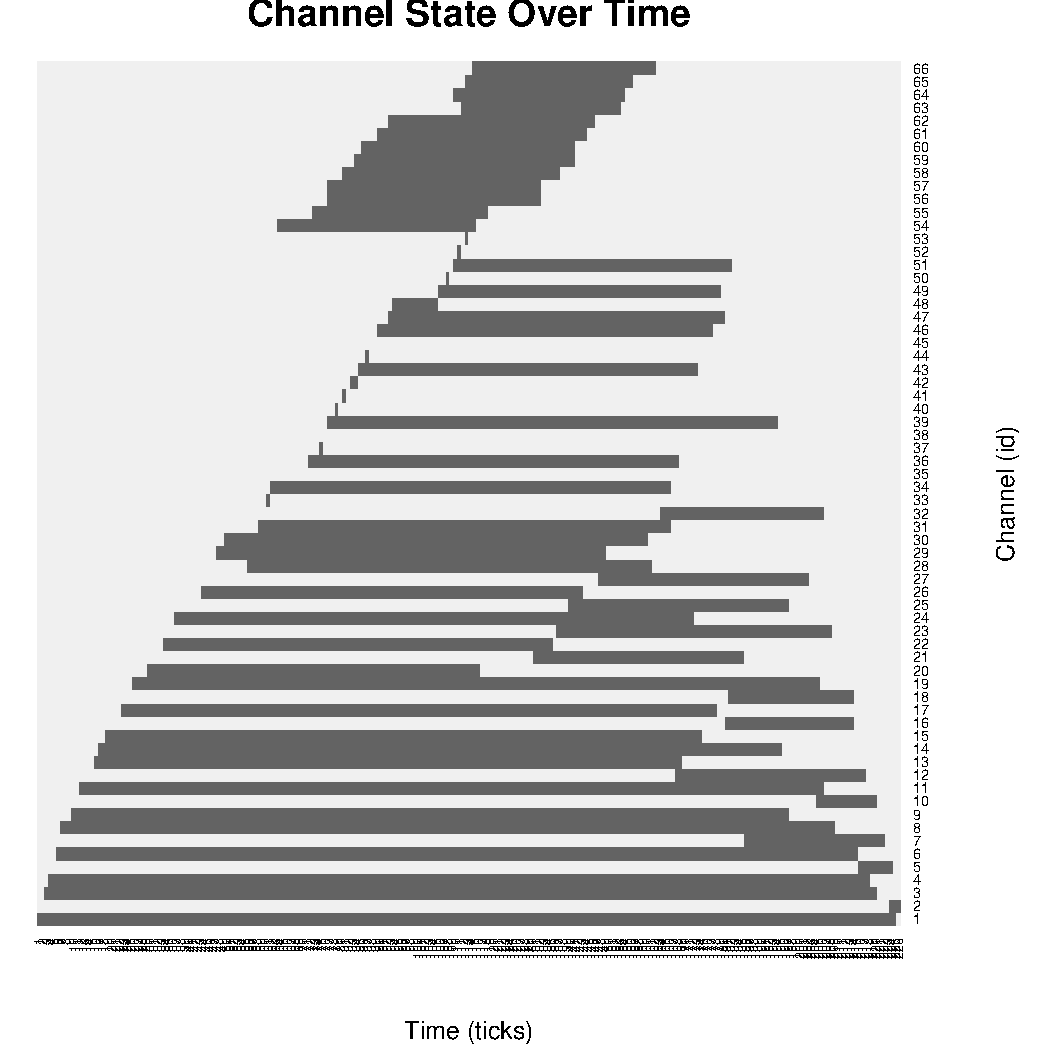
\includegraphics[scale=0.40]{fibonacci-channel-demo.pdf}
    \label{fig:fibonacci-channel-demo-chart}
}%
\subfigure{
    \centering
    \raisebox{20mm}{\footnotesize \BUseVerbatim{FibCode} }
\label{fig:fibonacci-channel-demo-code}
}
    \caption{Parallel Fibonacci implementation and a potential channel graph.}
    \label{fig:fibonacci-channel-demo}
\end{figure}

You may also note that the chart gives an indication as to the size of the time
quantum selected for the application's execution. The order in which a channel
becomes blocked, and it's order in the processes execution give that hint. The
large block of channels at the top of the graph indicate the last batch of 
spawned processes got time on the cpu before the one's which spawned it, as the
scheduler which evaluated the spawn ran out of reductions for that process. 
These observations will become useful for later scheduler critiques.

\subsection{Scheduler API}\label{sec:results-evaluation-classical}

The ErLam Scheduler API was minimally constructed around the single-step 
scheduling semantics presented earlier in figure~\ref{fig:scheduler-step}.
We were motivated by the simplicity of the description and thus the ability
to bring some formalism to the implementations. That being said, we would still
require the option to observe practical statistics such as runtime overhead 
during our scheduler comparisons. 

\begin{figure}[h!]
    \subfigure[Tick disparity, or the average time between scheduler ticks per 
    LPU, per Task run. Typical ranges tend to spike in groups, which show 
    consistency based on scheduler implementation, rather than OS intervention.]{
        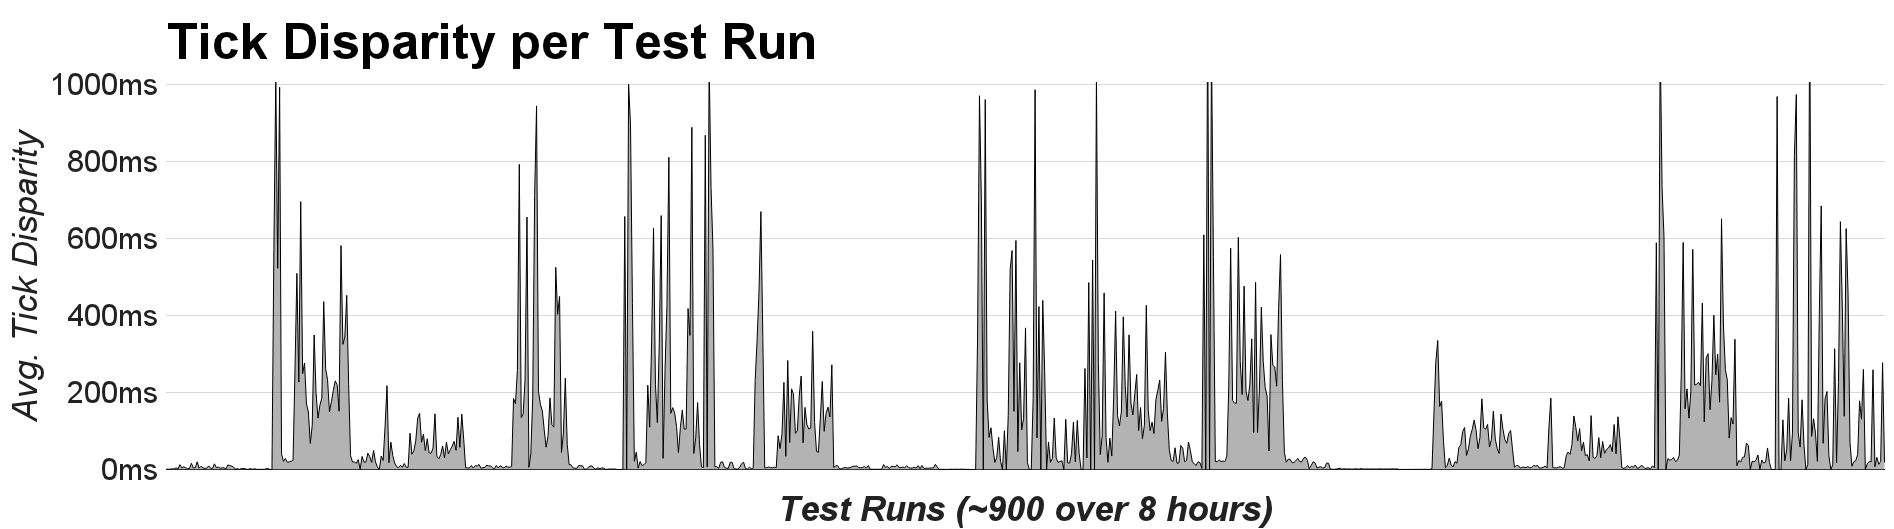
\includegraphics[width=\textwidth]{tick-disparity.png}
        \label{fig:tick-disparity}
    }
    \subfigure[Tick disparity consistently matches up with increased computation, 
    which is indicitive of inter-scheduler communication requirements.]{
        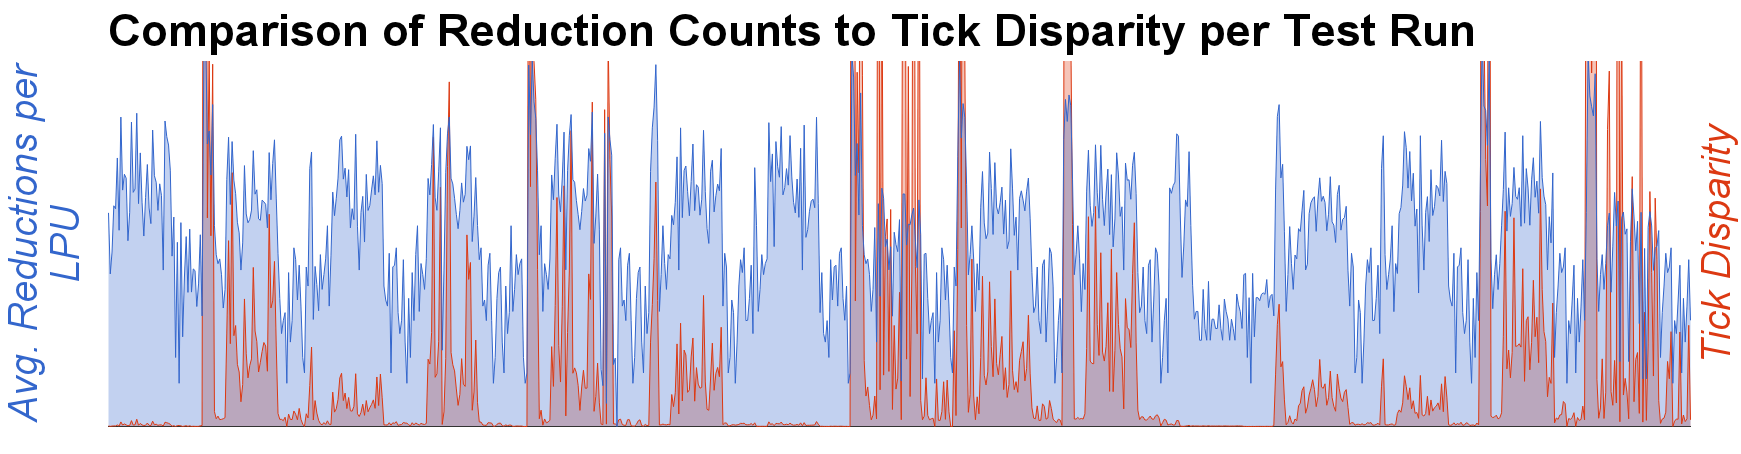
\includegraphics[width=\textwidth]{tick-disparity-to-reductions.png}
        \label{fig:tick-disparity-match}
    }
    \caption{Tick Disparity over nearly $900$ tests.}
\end{figure}

However,
wne of the concerns early on, and as described in section~\ref{sec:runtime log reports}, 
was that the LPUs could greatly differ in the number of ticks they are able to 
provide their process queue. This could be caused by the OS preempting the 
ErLam scheduling thread to execute something else. However, from our tests, we
found these gaps to be minimal and mainly caused by the scheduling implementation
itself. 

Figure~\ref{fig:tick-disparity} shows the average time between ticks averaged over
the LPUs for a large subsection of the tests we ran. We call this average time 
between ticks per LPU the Tick Disparity of the test. From the figure, we notice
obvious clustering, and figure~\ref{fig:tick-disparity-match} leads us to believe this
is primarily caused by spikes in reduction counts. A scheduler chugging on 
processes the entire time, must wait until preemption in-order to handle any 
inter-scheduler communication, as in the case of work-stealing schedulers. Thus,
for our purposes, all talk of tick-disparity could be considered a discussion of
scheduler overhead. As such, comparative analysis of scheduler implementation 
overhead from test case execution would still be a valid comparison with our
design.

Further, to validate that our scheduler implementations functioned as expected 
after translation was another concern. We gave the example of the CML 
Dual-Queue translation ($STDQ$) previously in section~\ref{sec:example the cml scheduler}.
We will now examine it's execution and compare it to $STRR$, a single queue naive
scheduler to confirm our understanding.

The key differences we would expect to see in a comparison would be that the CML
prefers to, and attempts to run the interactive processes first. It would push
all computational processes onto the secondary queue, only promoting them when 
the need arises. To observe this property, we compose the $UserInput_{(T,C)}$ 
test with $ChugMachine_N$ to create an interactivity test primitive 
$Interactivity_{(N,M)}$ (figure~\ref{fig:interactivity-code}). The primitive
launches $ChugMachine_N$ and $M$ instances of $UserInput_{(5,10)}$ (the values
of which were arbitrarily chosen so as to execute for long enough to collect
coherent data). We then subsequently ran this primitive with $STRR$ and $STDQ$
using multiple values for $N$ and $M$. Table~\ref{tab:interativity8-16-strr-stdq}
compares an instance of this test set: $Interactivity_{(8,16)}$.

\begin{table}[h]
    \begin{tabular}{@{}ccc}
$Interactivity_{(8,16)}$ & \textbf{$STRR$}       & \textbf{$STDQ$}       \\ \cline{2-3} 
\multicolumn{1}{c|}{\rotatebox{90}{\textbf{Channel State over Time}}} & 
    \multicolumn{1}{l|}{\includegraphics[scale=0.32]{tests/interactivity/single/pg_0001.pdf}} & 
    \multicolumn{1}{l|}{\includegraphics[scale=0.32]{tests/interactivity/cml/pg_0001.pdf}} \\ \cline{2-3} 
\multicolumn{1}{c|}{\rotatebox{90}{\textbf{Communication Density}}}   & 
    \multicolumn{1}{l|}{\includegraphics[scale=0.32]{tests/interactivity/single/pg_0002.pdf}} & 
    \multicolumn{1}{l|}{\includegraphics[scale=0.32]{tests/interactivity/cml/pg_0002.pdf}} \\ \cline{2-3} 
\multicolumn{1}{c|}{\rotatebox{90}{\textbf{Reduction Density}}}       & 
    \multicolumn{1}{l|}{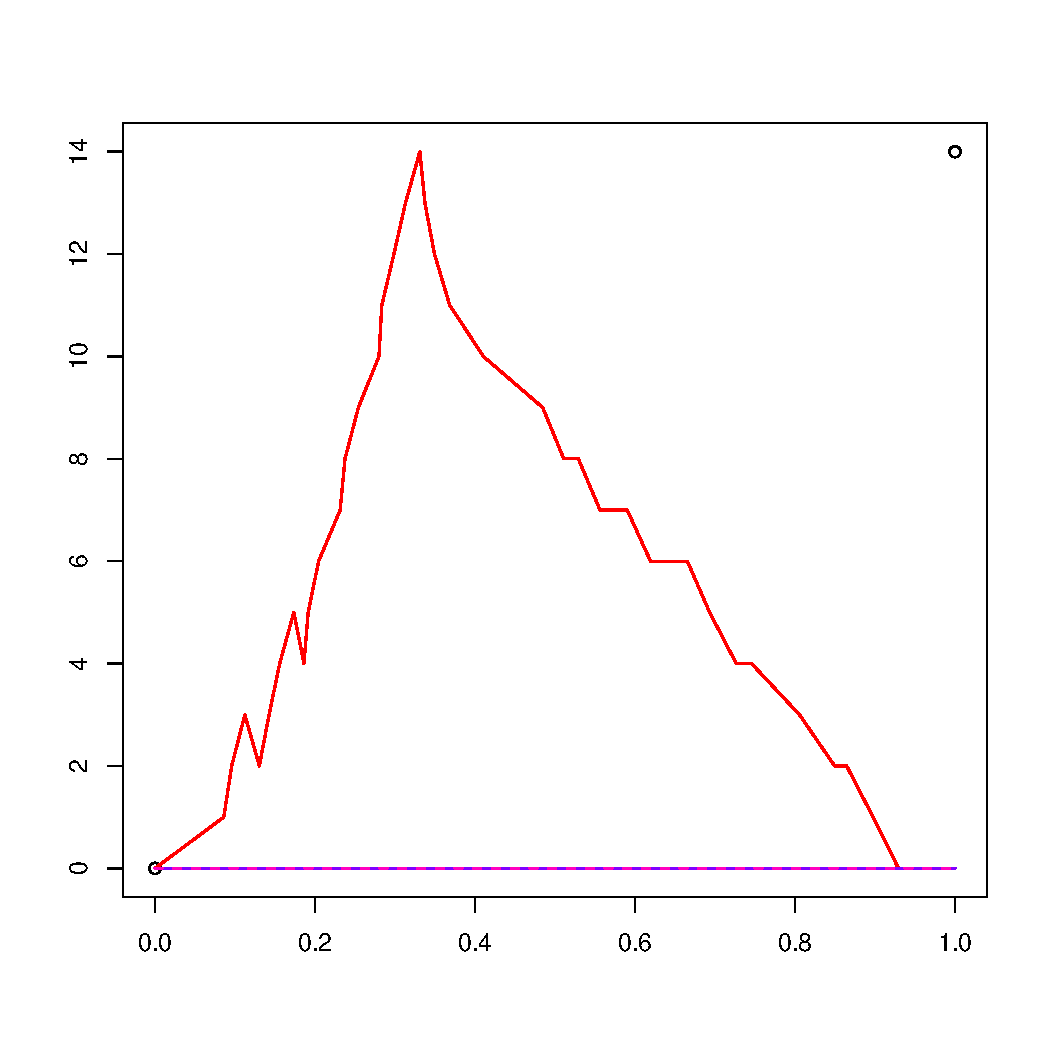
\includegraphics[scale=0.32]{tests/interactivity/single/pg_0003.pdf}} & 
    \multicolumn{1}{l|}{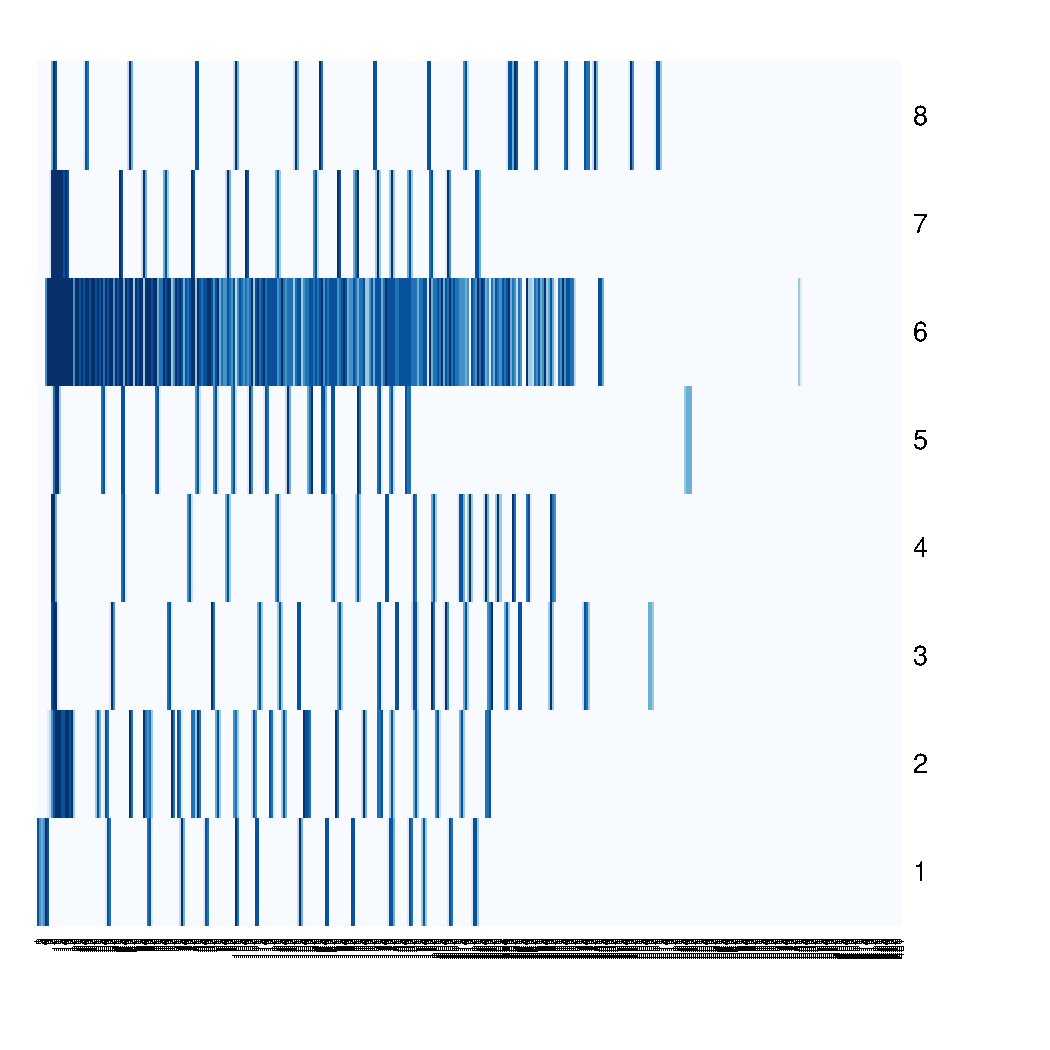
\includegraphics[scale=0.32]{tests/interactivity/cml/pg_0004.pdf}} \\ \cline{2-3} 
\end{tabular}
    \caption{Comparison of $STRR$ and $STDQ$ using Channel State, Reduction and Communication Densities.}
    \label{tab:interativity8-16-strr-stdq}
\end{table}

The Reduction Density graphs explain everything we need to know. The darkened portions
at the beginning of the chart indicate that the $STRR$ scheduler has no regard for the
interactive processes, whereas the $STDQ$ scheduler remains spread out. This seems to be
on the opposite if we were to consult the Communication Density charts though. It would appear
here that $STRR$ is getting more frequent communication, and $STDQ$ condenses all 
synchronizations to the end. This is however an issue of verbiage as Interactivity
does not correlate to Communication Density. By this we mean, $STRR$ is indeed allowing 
communication to happen evenly due to a round-robin schedule, but it is not attending to
spontanious events (\ie~responses back from $hang$). $STDQ$ on the otherhand pushes all 
inter-process communication backwards as it waits to respond to the $hang$ing processes.

We see this effect more clearly once we compare with the Channel State charts. In $STRR$
we see an even regard for all processes. The tapering of the channel blocks at the 
beginning of the graph is consistent with our understanding of the $merge$-based
successive spawning. However, $STDQ$ is completely different, and all $UserInput_{(T,C)}$
processes seem to be pushed to the beginning of the execution pool. This is infact due
to another difference between the execution styles of the two schedulers. $STDQ$ replaces
the currently running process with the child process it spawned, enqueuing the parent.
We therefore can confirm our understanding, in this case, that the scheduler is reacting
to the test primitives as expected.

\subsection{Channel Implementations}\label{sec:results-channel-implementations}

The above graphs (\eg~table~\ref{tab:interativity8-16-strr-stdq}) were generated, 
using the CML-like Process Absorption channels.

\todo[inline]{ There are 3 mechanisms provided by ErLam which modify the channel
  implementation: Blocking Channels, Absorption Channels, and then channel pinning
based on a spreading algorithm. In this section I'd primarily like to look at the
first two.
}
\subsection{Cooperativity Feedback Schedulers}\label{sec:results-evaluation-feedback}

\todo[inline]{ There are 3 schedulers, Longevity-Batcher, Channel-Pinner, Graph Shuffling.
I will primarily be looking at:\\

- How does Longevity Batcher degrade? Does it turn into MTRRWS?\\
- How quickly and thoroughly can Channel-Pinner saturate the cores with work?\\
- How does Graph Shuffling handle large and small process queues?
}


\section{Comparisons}\label{sec:results-comparisons}

Secondly, using our classical scheduler results as a base line we can evaluate 
the feedback schedulers independently. This will give an indication of what
may warrant further investigation, and testing. However, there are three 
questions which are of immediate interest:
\vspace{-3mm}\begin{itemize}
    \item Are there instances where the stealing mechanism matters?
    \item When does being cooperativity-conscious lead to better schedules?
    \item Does the overhead of feedback systems outweigh the benefits?
\end{itemize}

\todo[inline]{ Including the above, I will want to compare:\\
- MTRRWS-SQ and MTRRWS-IS \\
- STRR and MTRRGQ \\
- Long-Batcher and Channel-Pinner in terms of work-stealing \\
- All feedback schedulers in terms of: execution time (tick count), saturation, evenness of work-load.
}


\section{A Comment on Swap Channels}\label{sec:results-swap-channels}

Swap channels provided a number of benefits on the side of the language 
designer. They reduce the complexity of channel implementation, and as shown, 
they lend themselves to a number of possible designs. We demonstrated just two 
possible implementations, the Blocking and Absorption channels. As such, the 
concept of a swap channel as a language primitive is extremely attractive. 
However, swapping poses some problems for realistic applications which we would
now like to discuss.

\begin{figure}
\centering
\inputminted[frame=lines,fontsize=\footnotesize]{csharp}{code/badclustercomm.els}
\caption{A naive but ineffectual $ClusterComm_{(N,M)}$ implementation.} 
\label{fig:bad-clustercomm}
\end{figure}

First, a swap channel does not lend itself to a level of fairness that would be
expected by a programmer. We lead with our implementation of 
$ClusterComm_{(N,M)}$ as example, which due to being on top of swap channels, 
was made to be much more enigmatic. Figure~\ref{fig:bad-clustercomm} gives an
example implementation of $ClusterComm_{(N,M)}$. Note the third parameter to
the application, which denotes the number of time's each of the $N$ processes
should communicate. The system therefore blocks until all processes synchronize
$X$ times before quiting.

Due to this, we must pose several restrictions on the possible values of $N$ and
$M$. Namely, $N$ must be an even number, since all processes would need to have a 
partner to swap with, and $M$ must be no greater than $\lfloor N/2 \rfloor$, any
more and it would be possible for a process to hang indefinitely.

However, these two restrictions are not enough to guarantee the process terminates.
In fact, most runs of this application, with any value of $N > 2$ would most 
likely hang forever. This is due to the bias our program creates when spawning
processes, as well as the type of fairness the swap channel semantics provides.

First, our bias we introduce is merely because we cannot batch spawn a set of
processes at the same time. As such we will spawn one process at a time which
may get a chance to run before all others. As such the first several processes
may reach their synchronization limit before we are even done spawning the rest
of the processes. Due to this, we may have a case where all but $M$ processes
have completed, and thus all channels are blocked indefinitely.

Secondly, the channel semantics have no inherent preference for unseen 
or new processes. The scheduler may easily get in a loop of running the same
subset of processes repeatedly, this would have the same effect as the above
even if we were able to solve the bias problem. As such, this is inherently an
issue with the capabilities of swap channels. 

Thus, the best we can do for $ClusterComm_{(N,M)}$, is to run until at least 
$N-M$ processes have met their quota. Note this approach is only acceptable 
under Symmetric message passing constructs. In asymmetrical, even if there was
a guarantee of an equal number of senders and receivers, all senders could be
blocked on one channel while all receivers could be blocked on another. 

But this issue points to another problem with swap channels, insofar as they do
not lend themselves to being primitives at all. Due to this fairness issue, a 
language with swap channels would be unable to build the asymmetrical constructs
most user's would like. As such, they have been useful merely for simulation 
purposes.

However, for further simulation of cooperativity, it may be adventagous to also 
consider the directionality of communication. The recognition of consumer and 
producer processes may lend itself to further gains as the recognition of 
communication and computation bound processes did. This is not to say all gains
in utilizing pure synchronization have been obtained. 
